\documentclass[12pt, openany, oneside]{book}

\usepackage{listings}
\usepackage[dvipsnames]{xcolor}
\usepackage{ctex}
\usepackage{fontspec}
\usepackage{setspace}
\usepackage{tikz}
\usepackage{anyfontsize}
\usepackage{sectsty}
\usepackage{titlesec}
\usepackage{float}
\usepackage[hidelinks]{hyperref}
\usepackage[a4paper]{geometry}
\usepackage{url}
\usepackage{amssymb}
\usepackage{fontawesome5}
\usepackage[most]{tcolorbox}
\usepackage{stackengine}
\usepackage{multirow}
\usepackage{makecell}
\usepackage[T1]{fontenc}
\usepackage{diagbox}
\usepackage{longtable}
\usepackage{newtxtt}
\usepackage{pgf-umlcd}
\usepackage{pgf-umlsd}
\usepackage{bbding}
\usepackage{amsmath}
\usepackage[edges]{forest}
\usepackage{tkz-graph}
\usepackage{dcolumn}
\usepackage{tikzpeople}

\usetikzlibrary{calc,trees,positioning,arrows,fit,shapes}
\usetikzlibrary{shapes.multipart,chains}
\usetikzlibrary{shadows}
\usetikzlibrary{arrows.meta}
\usetikzlibrary{matrix,backgrounds}
\usetikzlibrary{automata}

\tikzset{block/.style={
        font=\sffamily,
        draw=black,
        thin,
        fill=pink!50,
        rectangle split,
        rectangle split horizontal,
        rectangle split parts=#1,
        outer sep=0pt},
        gblock/.style={
            block,
            rectangle split parts=#1,
            fill=green!30}
        }

\makeatletter
\newcommand{\verbatimfont}[1]{\renewcommand{\verbatim@font}{\ttfamily#1}}
\makeatother

\makeatletter
\def\BState{\State\hskip-\ALG@thistlm}
\makeatother

\def\rlwd{.5pt} \def\rlht{2.2ex} \def\rldp{.5ex}
\def\mydiv#1{~
  \rule[-\rldp]{\rlwd}{\rlht}
  \setbox0=\hbox{~#1}
  \stackunder[\dimexpr\rldp-\rlwd]{~#1}{\rule{\wd0}{\rlwd}}
}

\definecolor{mycolor}{RGB}{0,128,128}
\newtcbox{\mybox} {
    on line,
    colback=mycolor,
    fontupper=\bfseries\color{white},
    boxrule=0pt,
    arc=5pt, 
    boxsep=0pt, 
    left=2pt, 
    right=2pt, 
    top=5pt, 
    bottom=5pt
}

\setstretch{1.5}
\setlength{\parindent}{0cm}

\geometry{a4paper,top=2.5cm,bottom=2.5cm}

\titleformat{\chapter}{\Huge\Huge\bfseries}{\chaptertitlename\ \thechapter{\ }}{0pt}{\Huge}{}
\titlespacing{\chapter}{0pt}{0pt}{12pt}

\definecolor{dkgreen}{rgb}{0,0.4,0}
\definecolor{gray}{rgb}{0.5,0.5,0.5}
\definecolor{mauve}{rgb}{0.58,0,0.82}
\definecolor{LightGray}{gray}{0.9}

\lstset{
    basicstyle=\linespread{1.3} \fontspec{Consolas},    %  the size of the fonts that are used for the code
	basewidth=0.5em,
    numbers=left,            % where to put the line-numbers
    numberstyle=\color{black},  % the style that is used for the line-numbers
    numbersep=10pt,                  % how far the line-numbers are from the code
    backgroundcolor=\color{white},
    showspaces=false,
    showstringspaces=false,
    showtabs=false,
    frame=single,                   % adds a frame around the code
    rulecolor=\color{black},        % if not set, the frame-color may be changed on line-breaks within not-black text (e.g. commens (green here))
    tabsize=4,                      % sets default tabsize to 2 spaces
    captionpos=t,                   % sets the caption-position to bottom
    breaklines=false,                % sets automatic line breaking
    breakatwhitespace=true,        % sets if automatic breaks should only happen at whitespace
    title=\lstname,                   % show the filename of files included with \lstinputlisting;
    % also try caption instead of title
    numberstyle=\color{black},		% line number color
    keywordstyle=\color{blue},          % keyword style
    commentstyle=\color{dkgreen},       % comment style
    stringstyle=\color{mauve},         % string literal style
    escapeinside={\%*}{*)},            % if you want to add LaTeX within your code
    morekeywords={*,...}               % if you want to add more keywords to the set
}

\begin{document}

\thispagestyle{empty}

\begin{tikzpicture}[overlay,remember picture]
	\fill[
		black!2]
	(current page.south west) rectangle (current page.north east);

	\shade[
		left color=Dandelion,
		right color=Dandelion!40,
		transform canvas ={rotate around ={45:($(current page.north west)+(0,-6)$)}}]
	($(current page.north west)+(0,-6)$) rectangle ++(9,1.5);

	\shade[
		left color=lightgray,
		right color=lightgray!50,
		rounded corners=0.75cm,
		transform canvas ={rotate around ={45:($(current page.north west)+(.5,-10)$)}}]
	($(current page.north west)+(0.5,-10)$) rectangle ++(15,1.5);

	\shade[
		left color=lightgray,
		rounded corners=0.3cm,
		transform canvas ={rotate around ={45:($(current page.north west)+(.5,-10)$)}}] ($(current page.north west)+(1.5,-9.55)$) rectangle ++(7,.6);

	\shade[
		left color=orange!80,
		right color=orange!60,
		rounded corners=0.4cm,
		transform canvas ={rotate around ={45:($(current page.north)+(-1.5,-3)$)}}]
	($(current page.north)+(-1.5,-3)$) rectangle ++(9,0.8);

	\shade[
		left color=red!80,
		right color=red!80,
		rounded corners=0.9cm,
		transform canvas ={rotate around ={45:($(current page.north)+(-3,-8)$)}}] ($(current page.north)+(-3,-8)$) rectangle ++(15,1.8);

	\shade[
		left color=orange,
		right color=Dandelion,
		rounded corners=0.9cm,
		transform canvas ={rotate around ={45:($(current page.north west)+(4,-15.5)$)}}]
	($(current page.north west)+(4,-15.5)$) rectangle ++(30,1.8);

	\shade[
		left color=RoyalBlue,
		right color=Emerald,
		rounded corners=0.75cm,
		transform canvas ={rotate around ={45:($(current page.north west)+(13,-10)$)}}]
	($(current page.north west)+(13,-10)$) rectangle ++(15,1.5);

	\shade[
		left color=lightgray,
		rounded corners=0.3cm,
		transform canvas ={rotate around ={45:($(current page.north west)+(18,-8)$)}}]
	($(current page.north west)+(18,-8)$) rectangle ++(15,0.6);

	\shade[
		left color=lightgray,
		rounded corners=0.4cm,
		transform canvas ={rotate around ={45:($(current page.north west)+(19,-5.65)$)}}]
	($(current page.north west)+(19,-5.65)$) rectangle ++(15,0.8);

	\shade[
		left color=OrangeRed,
		right color=red!80,
		rounded corners=0.6cm,
		transform canvas ={rotate around ={45:($(current page.north west)+(20,-9)$)}}]
	($(current page.north west)+(20,-9)$) rectangle ++(14,1.2);

	% Title
	\node[align=center] at ($(current page.center)+(0,-7)$)
	{
	{\fontsize{60}{60} \selectfont {{软件工程}}}\\[1cm]
	{\fontsize{40}{40} \selectfont {{Software Engineering}}}\\[2cm]
	{\fontsize{20}{19.2} \selectfont \textcolor{orange}{ \bf 极夜酱}}\\[4pt]
	};
\end{tikzpicture}

\newpage

\pagestyle{plain}
\setcounter{page}{1}
\setcounter{tocdepth}{1}
\tableofcontents

\newpage

\setcounter{page}{1}

\chapter{需求工程}

\section{软件开发}

\subsection{软件开发}

什么是好的软件?一个好的软件需要满足三点要求:

\begin{enumerate}
    \item 一般要求(general requirements)
    \item 法律要求(legal requirements)
    \item 具体要求(specific requirements)
\end{enumerate}

一般要求包括软件系统需要有详细的文档、可读性高的代码、易于修改和维护的代码、能够开展测试、容易移植、使用方便等方面。\\

法律要求表示系统必须要遵守相关的法律法规。例如加拿大安大略省制定了残疾人无障碍法案,要求软件必须考虑照顾到残障人士的使用;加拿大反垃圾邮件立法规制了垃圾邮件、间谍软件、恶意软件和僵尸网络等问题。\\

具体要求即来自客户和用户具体的需求,软件系统应该要能够实现客户和用户提出的功能。\\

想要开发出一款好的软件,必须要拥有良好的编程能力,这可以通过大量练习提高。同时也需要具备良好的沟通和规划能力,例如在处理问题时,应该与客户或者熟悉问题的人沟通,确保理解了客户/用户的需求。编程前也可以先查找别人已经做过的相关内容,不要重复造轮子。

\newpage

\section{需求}

\subsection{用户故事(User Story)}

用户故事是用几句话描述用户会做的一件事,以及他们为什么要这样做。用户故事是关于用户将会做什么,而不是怎么做。\\

用户故事一般采用这样的格式:“As a [user type], I want [some action] so that [some reason].”。例如,“作为一个活跃用户,我想不用每次登录都输入账号密码,以便更方便快速地登录。”\\

\subsection{需求(Requirements)}

需求描述了软件做的某一件事,它可以是功能性(functional)或非功能性(non-functional)的。同样一个需求只需要描述做什么,而不是如何去做。\\

需求的作用是为了让开发者和客户都清楚最终产品想要的预期是什么。\\

一个好的需求应该具备以下条件:

\begin{itemize}
    \item 分类(categorized):使用MuSCOW法则对需求进行分类。
          \begin{itemize}
              \item MUSTS:系统能够满足客户的基本需求,类似于最小可行产品(minimum viable product)
              \item SHOULDS:满足客户基本或更高级的需求
              \item COULDS:能够使系统变得更好的额外需求
              \item WON'TS:系统不该做的事情
          \end{itemize}

    \item 有优先级(prioritized):对不同的需求指定一个优先级,需要遵守MUSTS > SHOULDS > COULDS > WONT'S。

    \item 逻辑合理:需求之间的依赖关系需要合理,例如一个MUST需求不能依赖于一个SHOULD需求。

    \item 时间估计(time estimate):一个需求应该需要在15天内完成,如果不能完成, 应该把它分解成多个小需求。
\end{itemize}

\newpage

\section{原型设计}

\subsection{原型设计(Prototyping)}

原型是指没有功能的模型,它不一定要包含一个程序的所有方面。\\

原型设计是与客户/用户沟通的一种工具,让客户/用户感觉他们自己也是设计者。原型设计的目的是为了验证UI是否能够可以被正常使用,让开发者能够以用户的角度思考问题。\\

\subsection{纸上原型(Paper Prototyping)}

纸上原型也称低保真原型(low fidelity prototyping),通过纸笔等工具设计,通常是UI设计的第一步。它具有制作过程快速、成本低、更改快速、效率高的特点。\\

\begin{figure}[H]
    \centering
    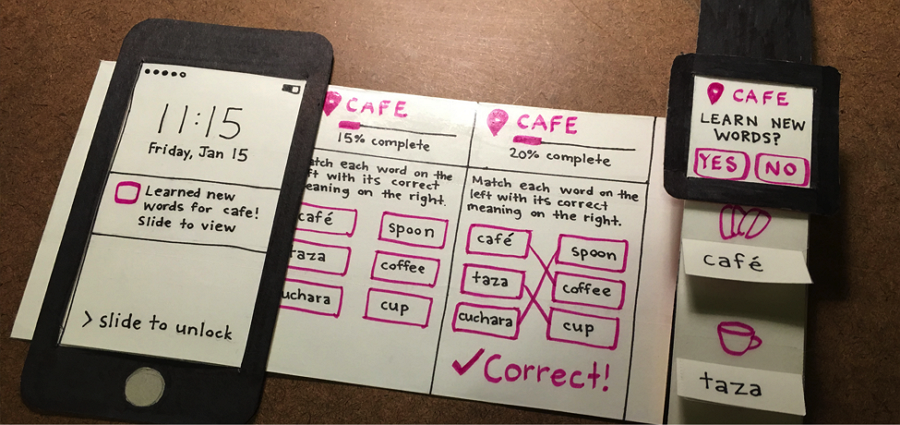
\includegraphics[scale=0.5]{img/C1/1-3/1.png}
    \caption{纸上原型}
\end{figure}

\begin{figure}[H]
    \centering
    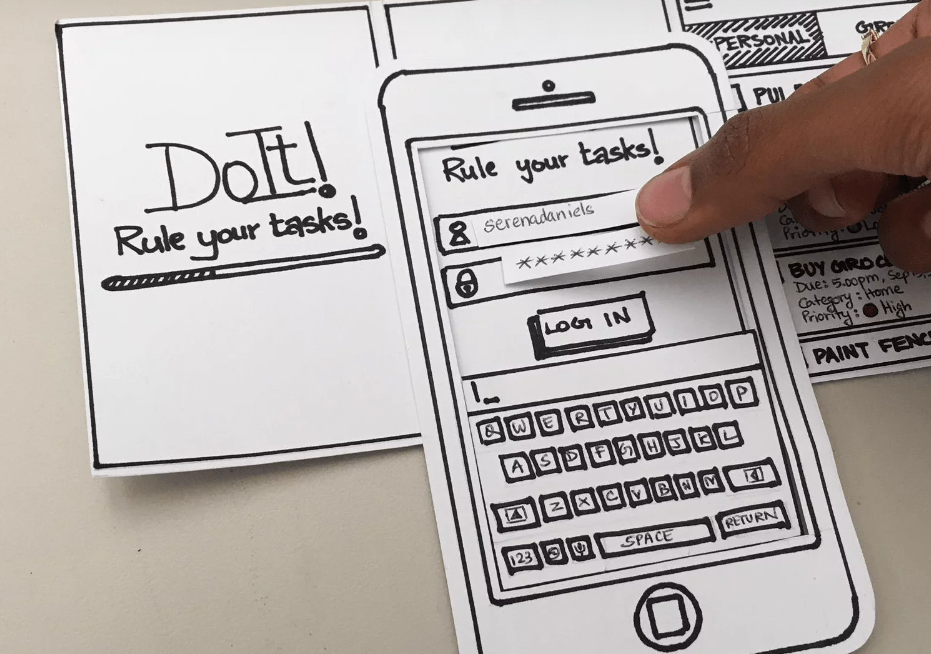
\includegraphics[scale=0.7]{img/C1/1-3/2.png}
    \caption{纸上原型}
\end{figure}

纸上原型的目的并不是为了让UI更加美观,而是为了确保系统的流程是否存在问题。\\

在完成纸上原型后,需要让参与测试的人根据用例进行测试。在测试过程中,不要提供任何帮助或者指导,以此来验证用户交互是否流畅。\\

最后,记录下在纸上原型测试中哪些地方是正常的、哪些地方存在问题或遗漏的。\\

\subsection{线框图(Wireframing)}

线框图也称高保真原型(high fidelity prototyping),它看上去非常接近最终产品,几乎完全按照实物来制作,原型中甚至包含产品的细节、真实的交互、UI等。\\

\begin{figure}[H]
    \centering
    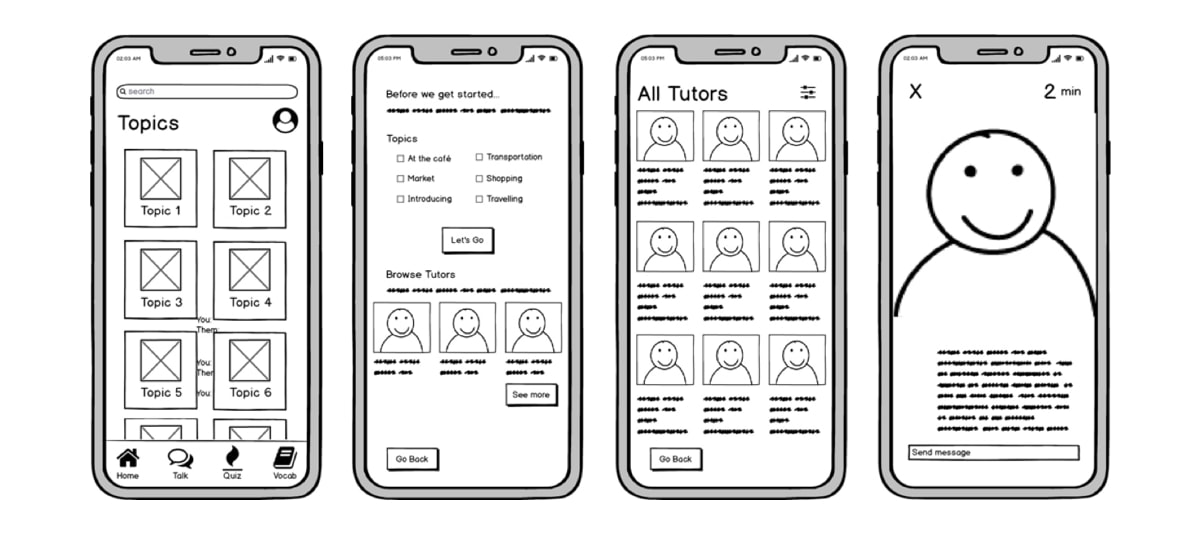
\includegraphics[scale=0.35]{img/C1/1-3/3.png}
    \caption{线框图}
\end{figure}

\begin{figure}[H]
    \centering
    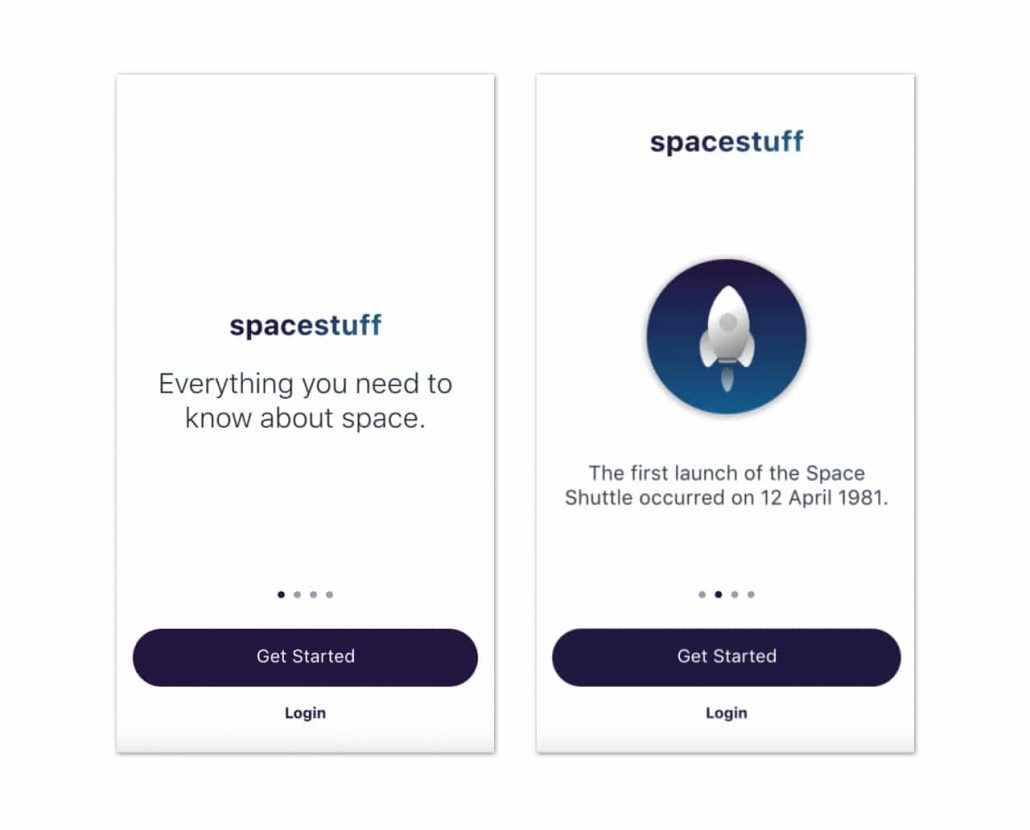
\includegraphics[scale=0.5]{img/C1/1-3/4.png}
    \caption{线框图}
\end{figure}

高保真原型的目的在于让用户提供反馈,例如UI中控件的位置和UI的美观程度。

\newpage
\chapter{软件过程}

\section{软件过程模型}

\subsection{瀑布模型(Waterfall)}

软件工程是使用系统化的、严格约束的、可量化的方法开发、运行和维护软件。\\

瀑布模型是一个软件生命周期模型,开发过程是通过一系列阶段顺序开展的,从系统需求分析直到产品发布,项目开发从一个阶段流动到下一阶段,这也是瀑布模型名称的由来。直到80年代早期,它一直是唯一被广泛采用的软件开发模型。\\

\begin{figure}[H]
    \centering
    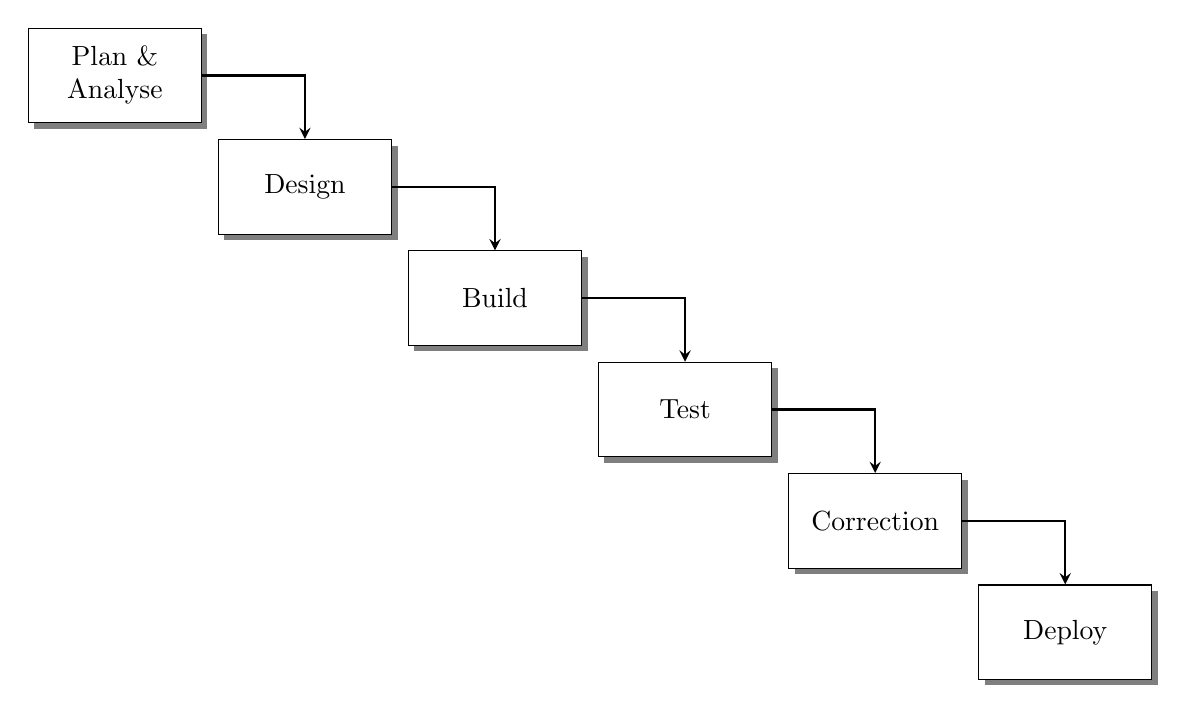
\begin{tikzpicture}[>=stealth,
            node distance = 2mm and 2mm,
            start chain = A going below right,
            every node/.style = {draw, text width=20mm, minimum height=12mm, align=center,
                    inner sep=1mm, fill=white, drop shadow={fill=black}, on chain=A},
        ]

        \node {Plan \& Analyse};
        \node {Design};
        \node {Build};
        \node {Test};
        \node {Correction};
        \node {Deploy};

        \foreach \i [count=\j] in {2,...,6}
            {
                \draw[->, thick] (A-\j) -| (A-\i);
            }
    \end{tikzpicture}
    \caption{瀑布模型}
\end{figure}

瀑布模型的特点是各阶段间具有顺序性和依赖性,必须等前一阶段的工作完成之后,才能开始后一阶段的工作。前一阶段的输出文档就是后一阶段的输入文档。\\

因此,瀑布模型是由文档驱动的,在可运行的软件产品交付给用户之前,用户只能通过文档来了解产品。瀑布模型几乎完全依赖于书面的规格说明,很可能导致最终开发出的软件产品不能真正满足用户的需要。也不适合需求模糊的系统。\\

传统的瀑布模型过于理想化,人在工作过程中不可能不犯错误。因而产生了 加入迭代过程的瀑布模型。\\

\begin{figure}[H]
    \centering
    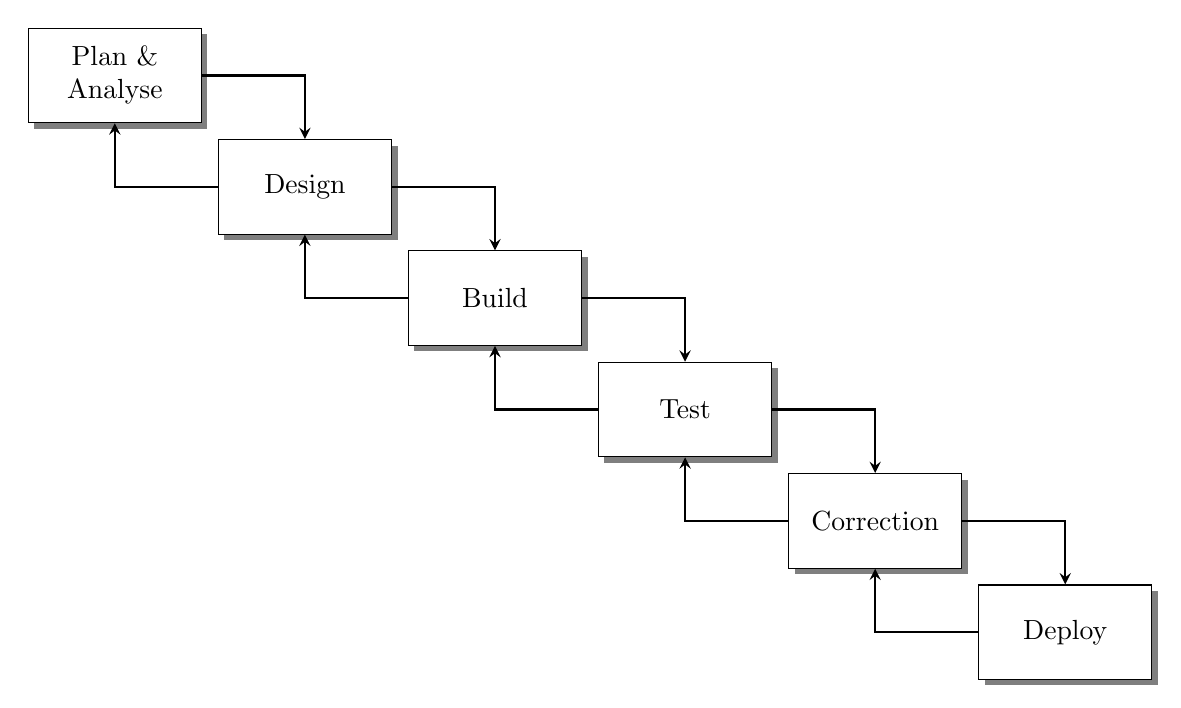
\begin{tikzpicture}[>=stealth,
            node distance = 2mm and 2mm,
            start chain = A going below right,
            every node/.style = {draw, text width=20mm, minimum height=12mm, align=center,
                    inner sep=1mm, fill=white, drop shadow={fill=black}, on chain=A},
        ]

        \node {Plan \& Analyse};
        \node {Design};
        \node {Build};
        \node {Test};
        \node {Correction};
        \node {Deploy};

        \foreach \i [count=\j] in {2,...,6}
            {
                \draw[->, thick] (A-\j) -| (A-\i);
                \draw[->, thick] (A-\i) -| (A-\j);
            }
    \end{tikzpicture}
    \caption{加入迭代过程的瀑布模型}
\end{figure}

\vspace{0.5cm}

\subsection{增量式开发(Incremental Development)}

\begin{figure}[H]
    \centering
    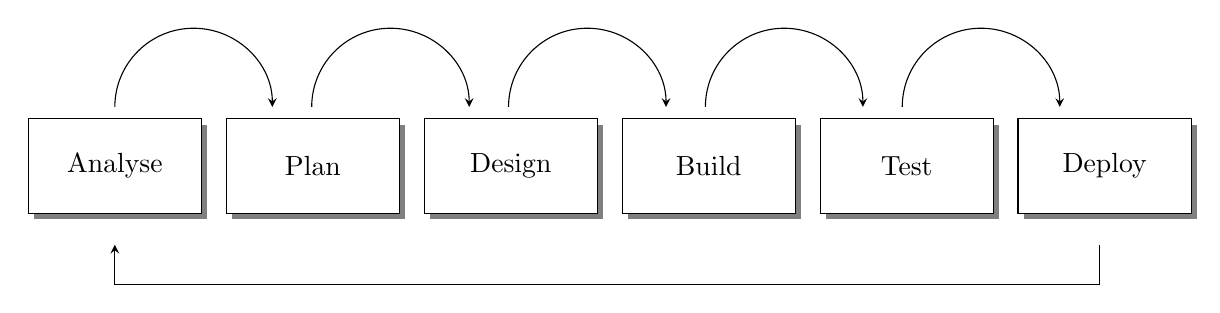
\begin{tikzpicture}[>=stealth,
        node distance = 3mm and 3mm,
        start chain = A,
        every node/.style = {draw, text width=20mm, minimum height=12mm, align=center,
                inner sep=1mm, fill=white, drop shadow={fill=black}, on chain=A},
    ]
        \node {Analyse};
        \node {Plan};
        \node {Design};
        \node {Build};
        \node {Test};
        \node {Deploy};

        \draw[->] (0,0.75) arc (180:0:1);
        \draw[->] (2.5,0.75) arc (180:0:1);
        \draw[->] (5,0.75) arc (180:0:1);
        \draw[->] (7.5,0.75) arc (180:0:1);.
        \draw[->] (10,0.75) arc (180:0:1);
        \draw[->] (12.5,-1) -- (12.5,-1.5) -- (0,-1.5) -- (0,-1);
    \end{tikzpicture}
    \caption{增量式开发}
\end{figure}

增量式开发允许开发人员加以利用系统的早期交付版本,重新参考和修改以达到预期的结果。增量式开发较为灵活快速,在开发的每个周期都会产出一个能够交付的版本。这样较为频繁的交付,能够使客户持续地提供反馈,从而获得更高质量的产品。

\newpage

\section{敏捷开发}

\subsection{敏捷开发(Agile)}

推行新的软件过程模型的原因在于,传统的开发方式有着更高的失败率,大部分项目的支出都远超出预算水平。\\

很多项目的开发阶段都超出了预期的时间,同时由于软件开发的特性,反而会导致"Adding people to a late project just makes it later"。\\

敏捷开发方法是一种将精力集中在软件本身,而不是设计和文档上。它依赖迭代的方法来完成软件的描述、开发和交付。\\

敏捷方法的核心思想体现在:

\begin{itemize}
    \item Individuals and interactions over processes and tools.
    \item Working software over comprehensive documentation.
    \item Customer collaboration over contract negotiation.
    \item Responding to change over following a plan.
\end{itemize}

这些思想主要表现为注重客户的参与,客户会在开发过程中紧密参与,为软件系统提供新的需求和评估。同时敏捷开发要求能够接受变更,设计的系统需要能够适应新的需求变化。\\

\subsection{敏捷项目管理}

Scrum方法是一个通用的敏捷方法,它更加注重迭代开发的管理。\\

在Scrum中,每个开发周期都包含开发任务的分配、实现、当前版本演示和会议讨论。每个周期都有一个固定的长度,通常为2$ \sim $4周,每个周期开发者会根据开发任务的清单,依据需求的优先级各自实现需求。在该周期无法完成的任务,会被继续放入任务清单,在下个周期继续完成。\\

在每个周期结束后,项目团队的所有成员需要参加会议讨论,根据当前版本的软件,回顾开发过程、交流问题等。\\

Scrum使得产品被分解为多个可管理的部分,整个团队所做的任务都是可见的,有助于改善团队见的沟通。同时也能阶段性地交付产品给用户,在下个周期能够根据用户反馈进行修改。

\newpage
\chapter{UML}

\section{UML}

\subsection{UML(Unified Modeling Language)}

统一建模语言UML是一种为面向对象系统的产品进行说明、可视化和编制文档的一种标准语言。\\

UML中包含了一系列不同类型的图:

\begin{itemize}
    \item 类图
    \item 组件图
    \item 部署图
    \item 对象图
    \item 封装图
    \item 复合结构图
    \item 剖面图
    \item 用例图
    \item 活动图
    \item 状态机图
    \item 序列图
    \item 通讯图
    \item 交互概览图
    \item 时序图
\end{itemize}

这些图主要可分为三大类:

\begin{enumerate}
    \item 功能模型(functional model):从用户的角度展示系统的功能,如用例图。
    \item 对象模型(object model):采用对象、属性、操作、关联等展示系统的结构,如类图、对象图。
    \item 动态模型(dynamic model):展现系统的内部行为,如时序图、活动图、状态图。
\end{enumerate}

\newpage

\section{用例图}

\subsection{用例图(Use Case Diagram)}

用例图用于描述从用户角度所看到的系统功能。通过用例图,人们可以获知系统不同种类的用户和用例。\\

\begin{figure}[H]
    \centering
    \begin{tikzpicture}
        \draw (0,0) rectangle (6,17);
        \node at (1.5,16.5) {Bank ATM};
        \draw (3,14.5) ellipse (2 and 1) node {查看余额};
        \draw (3,12) ellipse (2 and 1) node {存款};
        \draw (3,9.5) ellipse (2 and 1) node {取款};
        \draw (3,7) ellipse (2 and 1) node {转账};
        \draw (3,4.5) ellipse (2 and 1) node {维护};
        \draw (3,2) ellipse (2 and 1) node {维修};

        \draw (-3,13) circle (0.25);
        \draw (-3.5,12.5) -- (-2.5,12.5);
        \draw (-3,12.75) -- (-3,12);
        \draw (-3,12) -- (-3.5,11.5);
        \draw (-3,12) -- (-2.5,11.5);
        \node at (-3,11) {客户};

        \draw (-3,6) circle (0.25);
        \draw (-3.5,5.5) -- (-2.5,5.5);
        \draw (-3,5.75) -- (-3,5);
        \draw (-3,5) -- (-3.5,4.5);
        \draw (-3,5) -- (-2.5,4.5);
        \node at (-3,4) {技术人员};

        \draw (9,8.5) circle (0.25);
        \draw (9.5,8) -- (8.5,8);
        \draw (9,8.25) -- (9,7.5);
        \draw (9,7.5) -- (9.5,7);
        \draw (9,7.5) -- (8.5,7);
        \node at (9,6.5) {银行};

        \draw (-2,12.5) -- (1,14.5);
        \draw (-2,12.5) -- (1,12);
        \draw (-2,12.5) -- (1,9.5);
        \draw (-2,12.5) -- (1,7);

        \draw (-2,5.5) -- (1,4.5);
        \draw (-2,5.5) -- (1,2);

        \draw (8,8.5) -- (5,14.5);
        \draw (8,8.5) -- (5,12);
        \draw (8,8.5) -- (5,9.5);
        \draw (8,8.5) -- (5,7);
        \draw (8,8.5) -- (5,4.5);
        \draw (8,8.5) -- (5,2);
    \end{tikzpicture}
    \caption{银行ATM系统}
\end{figure}

\newpage

\section{类图}

\subsection{类图(Class Diagram)}

类图用于显示模型的静态结构,例如类的内部结构以及类与类之间的关系。\\

一个类包含属性和方法两部分,在类图中public属性和方法使用“+”表示,private属性和方法使用“-”表示,protected属性和方法使用“\#”表示。\\

\begin{figure}[H]
    \centering
    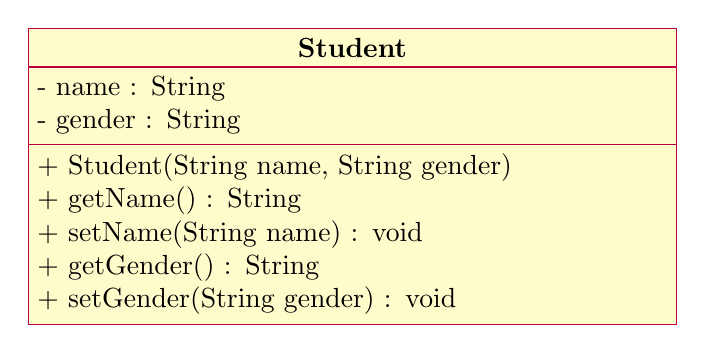
\begin{tikzpicture}
        \begin{class}[text width = 8cm]{Student}{0,0}
            \attribute{- name : String}
            \attribute{- gender : String}
            \operation{+ Student(String name, String gender)}
            \operation{+ getName() : String}
            \operation{+ setName(String name) : void}
            \operation{+ getGender() : String}
            \operation{+ setGender(String gender) : void}
        \end{class}
    \end{tikzpicture}
    \caption{Student类}
\end{figure}

\vspace{0.5cm}

\subsection{继承(Inheritance)}

\begin{figure}[H]
    \centering
    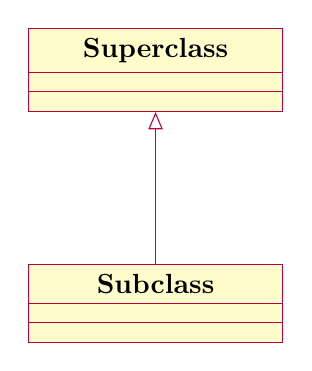
\begin{tikzpicture}
        \begin{class}[text width = 3cm]{Superclass}{0,0}
        \end{class}

        \begin{class}[text width = 3cm]{Subclass}{0,-3}
            \inherit{Superclass}
        \end{class}
    \end{tikzpicture}
    \caption{继承}
\end{figure}

子类和父类之间存在“is a”的关系,例如Dog和Cat都属于Animal的子类。\\

\subsection{关联(Association)}

\begin{figure}[H]
    \centering
    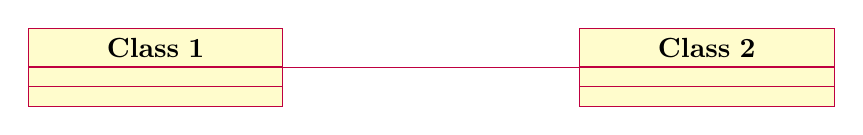
\begin{tikzpicture}
        \begin{class}[text width = 3cm]{Class 1}{0,0}
        \end{class}

        \begin{class}[text width = 3cm]{Class 2}{7,0}
        \end{class}

        \association {Class 1}{}{}{Class 2}{}{}
    \end{tikzpicture}
    \caption{关联}
\end{figure}

关联关系使一个类能够知道另一个类的属性和方法。关联可以是双向的,也可以是单向的。\\

关联关系还可以指定多重性(multiplicity)。例如一个Student可以和多个Professor存在关联。\\

\begin{figure}[H]
    \centering
    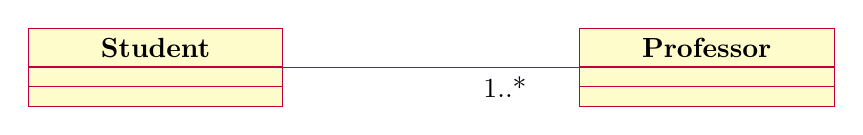
\begin{tikzpicture}
        \begin{class}[text width = 3cm]{Student}{0,0}
        \end{class}

        \begin{class}[text width = 3cm]{Professor}{7,0}
        \end{class}

        \association {Student}{}{}{Professor}{}{1..*}
    \end{tikzpicture}
\end{figure}

一个Professor可以和多个Student存在关联。\\

\begin{figure}[H]
    \centering
    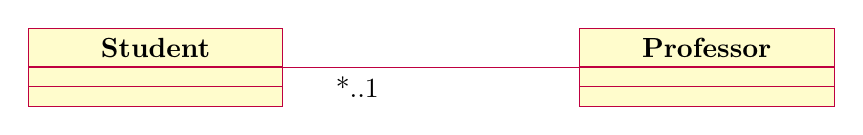
\begin{tikzpicture}
        \begin{class}[text width = 3cm]{Student}{0,0}
        \end{class}

        \begin{class}[text width = 3cm]{Professor}{7,0}
        \end{class}

        \association {Student}{}{*..1}{Professor}{}{}
    \end{tikzpicture}
\end{figure}

多个Professor同样也可以和多个Student存在关联。\\

\begin{figure}[H]
    \centering
    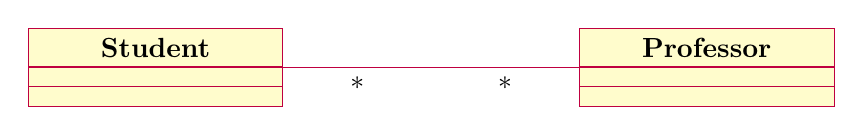
\begin{tikzpicture}
        \begin{class}[text width = 3cm]{Student}{0,0}
        \end{class}

        \begin{class}[text width = 3cm]{Professor}{7,0}
        \end{class}

        \association {Student}{}{*}{Professor}{}{*}
    \end{tikzpicture}
\end{figure}

\vspace{0.5cm}

\subsection{聚合(Aggregation)}

聚合关系是关联联系的特例,用于表示整体和部分的关系,即“has a”。但是整体和部分有各自独立的生命周期。\\

例如Monther有一个Child,但是如果Mother死了,Child仍然存活。\\

\begin{figure}[H]
    \centering
    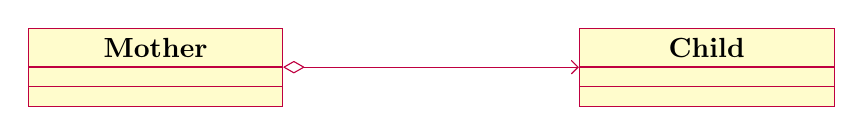
\begin{tikzpicture}
        \begin{class}[text width = 3cm]{Mother}{0,0}
        \end{class}

        \begin{class}[text width = 3cm]{Child}{7,0}
        \end{class}

        \aggregation {Mother}{}{}{Child}
    \end{tikzpicture}
    \caption{聚合}
\end{figure}

\vspace{0.5cm}

\subsection{组合(Composition)}

组合用于表示“part of”的的关系,因此具有组合关系的两个类具有相同的声明周期。\\

例如血液细胞是身体的一部分,人死了,血液细胞也会死。\\

\begin{figure}[H]
    \centering
    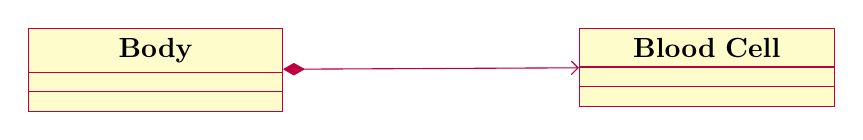
\begin{tikzpicture}
        \begin{class}[text width = 3cm]{Body}{0,0}
        \end{class}

        \begin{class}[text width = 3cm]{Blood Cell}{7,0}
        \end{class}

        \composition {Body}{}{}{Blood Cell}
    \end{tikzpicture}
    \caption{组合}
\end{figure}

\newpage

\section{时序图}

\subsection{时序图(Sequence Diagram)}

时序图通过描述对象之间发送消息的时间顺序显示多个对象之间的动态协作。\\

时序图中包括以下元素:

\begin{enumerate}
    \item 角色(actor)/对象(object):系统角色,可以是人或者其它子系统。

    \item 生命线(lifeline):表示对象在一段时期内的存在。

    \item 控制焦点(activation):在时序图中每条生命线上的窄矩形代表活动期。

    \item 消息(message):类角色通过发送和接受信息进行通信。
\end{enumerate}

\begin{figure}[H]
    \centering
    \begin{sequencediagram}
        \newthread{computer}{:Computer}
        \newinst[3]{server}{:Server}

        \begin{messcall}{computer}{sendEmail()}{server}
        \end{messcall}

        \postlevel\postlevel

        \begin{call}{computer}{newEmail()}{server}{response}
        \end{call}

        \postlevel\postlevel

        \begin{messcall}{computer}{deleteEmail()}{server}
        \end{messcall}
    \end{sequencediagram}
    \caption{时序图}
\end{figure}

\newpage
\chapter{}

\section{}

\subsection{}
\chapter{软件质量}

\section{软件质量}

\subsection{软件质量(Software Quality)}

一个质量好的软件从一个优秀的团队和开发过程开始,并且正确地使用系统架构和设计模式,后期严格的审查和测试都能够有效地增加软件的质量。\\

软件质量的特征包括:

\begin{itemize}
    \item 功能性
    \item 可靠性
    \item 易使用性
    \item 效率
    \item 可维护性
    \item 可移植性
\end{itemize}

客户/用户而言,他们的满足度取决于软件的质量、产品的一致性和是否在预算和预期时间内交付。\\

一个高质量的软件应该符合以下特征:

\begin{itemize}
    \item 易于使用
    \item 保证安全和隐私
    \item 较少的维护成本
    \item 较少的bug
    \item 客户满意度所带来的收益
    \item 在未来的产品中可以复用技术
\end{itemize}

\vspace{0.5cm}

\subsection{软件质量保证(SQA/QA, Software Quality Assurance)}

一个公司通常有一个独立的SQA小组与开发团队合作,评估正在生产的产品质量。即使在软件开发过程中注重错误的预防,也不能减少对QA的需求。\\

SQA小组的职责主要包括:

\begin{itemize}
    \item 准备SQA计划:评估标准、审查、错误跟踪。
    \item 协助开发过程:分析软件的缺陷和流程。
\end{itemize}

\newpage

\section{缺陷预防}

\subsection{代码评审(Code Review)}

软件缺陷很大一部分是来自于对需求的定义和理解不正确,code review是最有效的去除缺陷的手段。越早去除这些潜在的缺陷,所需的代价也越小。\\

Code review不是为了去刻意批斗某个开发者,而是为了团队成员之间相互了解学习,加深成员对系统的理解,使团队成员的代码更加健壮,提早发现代码缺陷。\\

Code review由一组技术人员组成,主要是为了发现软件中功能和逻辑的漏洞,验证功能是否满足了客户/用户的需求,保持项目的可维护性。\\

在code review过程中,可以根据检查清单(checklist)对产品进行检查,并记录下存在的问题。Code review的目的在于发现问题,而不是解决问题。\\

Code review的好处包括:

\begin{itemize}
    \item 提升系统的可维护性

    \item 及早发现潜在bug,降低事故成本。

    \item 促进团队内部知识共享,提高团队整体水平。

    \item 对于评审人员来说是一种思路重构的过程,可以帮助更多的人理解系统。

    \item 彼此能熟悉对方模块。
\end{itemize}

\newpage

\section{缺陷检测}

\subsection{缺陷检测(Defect Detection}

缺陷检测包括三个过程:

\begin{enumerate}
    \item 测试(testing):根据测试用例发现错误。
    \item 调试(debugging):查找并消除故障的原因。
    \item 监控(monitoring):监视有关状态和行为的信息。
\end{enumerate}

缺陷检测可以通过静态分析(static analysis)和动态分析(dynamic analysis)两种方式进行。\\

静态分析包括code review、向他人解释代码流程、借助自动化的工具检查语法语义错误及代码规范。\\

动态分析包括:

\begin{itemize}
    \item 黑盒测试(black-box testing):测试子系统的输入/输出行为。
    \item 白盒测试(white-box testing):测试子系统或类的内部逻辑。
\end{itemize}

\vspace{0.5cm}

\subsection{测试}

测试最好是由非开发软件的人进行,因为开发者一般会更加注重能够使程序正常工作的数据。当其他人使用程序时,往往会发现程序的问题。\\

因此一个测试人员非常有必要对系统由足够的了解,掌握各种测试方法和技术。\\

测试分为4种类型:

\begin{enumerate}
    \item 单元测试(unit testing):对每个类/子系统单独测试,确保每个模块的正确性。

    \item 集成测试(integration testing):将模块组装成子系统,确保各个模块连接在一起后也能正常工作。

    \item 系统测试(system testing):对整个系统进行测试。

    \item 验收测试(acceptance test):由客户/用户进行测试。
\end{enumerate}

\end{document}